\documentclass[g5paper,10pt,final,openright,coverpage,swedish]{thesis}

%% Standard packages
\usepackage{xcolor}
\usepackage{graphicx}
\usepackage{amsmath}
\usepackage{pdfpages}
\usepackage{booktabs}
\usepackage[hidelinks]{hyperref}

%% For demo text
\usepackage{lipsum}

%% Epigraph
\usepackage{epigraph}
\makeatletter
   \let\@epipart\@endpart
   \renewcommand{\@endpart}{\thispagestyle{epigraph}\@epipart}
\makeatother         
\setlength\epigraphwidth{\textwidth}

%% Glossary
\usepackage[acronym,
nomain,
nonumberlist,
nopostdot]{glossaries}
\makeglossaries

%% Bibliography
\usepackage[citestyle=authoryear,
bibstyle=authoryear,
sorting=nyt,
backend=bibtex,
natbib]{biblatex}
\addbibresource{bibliography.bib}
\setlength\bibitemsep{0.5\baselineskip}

%% Sections with no indent
\newenvironment{zeroindent}
{\par\setlength{\parindent}{0pt}}
{\par}

%% Document information 
\title{Thesis title}
\author{Your Name}
\date{May 2020}
\shortdate{2020}
\type{Doctoral Thesis in Physics}
\division{Particle and Astroparticle Physics}
\department{Department of Physics}
\address{SE-106 91 Stockholm, Sweden}
\city{Stockholm}
\country{Sweden}
\publisher{Printed by Universitetsservice US-AB}
\copyrightline{\copyright\ Your Name, May 2020}
\trita{Get from administration/online}
\isbn{Get from administration/online}
\cplogo{images/kth_logo.png}
\cplogonblines{1} % Number of text lines below kth logo... don't ask..
\cpillustration{images/nyan_cat.png} % Front page image
\innerlogo{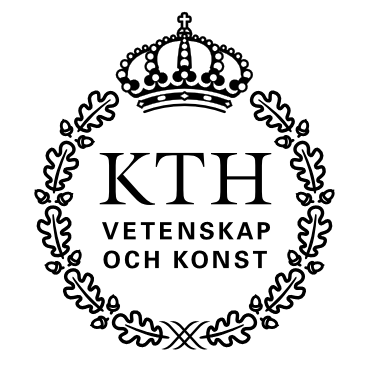
\includegraphics[width=32mm]{images/kth_logo.png}}
\centercomment{Cover illustration: Nyan cat} 
\foregincomment{Akademisk avhandling som med tillst{\aa}nd av Kungliga Tekniska h{\"o}gskolan i Stockholm framl{\"a}gges till offentlig granskning f{\"o}r avl{\"a}ggande av teknologie doktorsexamen [date, time, and place], AlbaNova Universitetscentrum, Roslagstullsbacken 21, Stockholm.\\ \\ Avhandlingen f{\"o}rsvaras p{\aa} engelska.}

%% MAIN DOCUMENT %%
\begin{document}

\maketitle

\cleardoublepage

%% Abstract

\chapter{Abstract}
\label{ch:abstract}

\lipsum[1]

%% Sammanfattning

\chapter{Sammanfattning}
\label{ch:sammanfattning}

\lipsum[1]


\tableofcontents

%% Introduction

\chapter{Introduction}
\label{ch:intro}

\lipsum[10-20]

%% Paper summary

\chapter{\label{ch:paper_summary}Publication list}

\begin{zeroindent}

  \section*{Publications included in the thesis}
  
  \subsection*{Paper~I}

  \textbf{Name, A.} et al., 2020, Article title. \textit{Journal}, 10, 99.

  \href{https://doi.org/}{\texttt{DOI}}

  \href{https://arxiv.org/}{\texttt{arXiv:identifier}}

  \subsection*{Paper~II}  


  \subsection*{Paper~III}

  
  
  \section*{Additional publications not included in the thesis}

  \subsection*{Paper~4}


  \subsection*{Paper~5}


  \subsection*{Paper~6}
  
  
\end{zeroindent}


%% Author contribution

\chapter{\label{ch:author_contribution}Author's contribution}

\lipsum[21]

\begin{zeroindent}

  \subsection*{Paper~I}
  \lipsum[22]  
  
  \subsection*{Paper~II}
  \lipsum[23]
  
  \subsection*{Paper~III}
  \lipsum[24]
  
\end{zeroindent}


%% Acknowledgements

\chapter{Acknowledgements}
\lipsum[25-28]

% This separates the introduction from the main part of the thesis.
\mainmatter

%% Chapters
\cleardoublepage

%% Part I

\epigraphhead[350]{\centering \textit{I'm the most influential man in footwear right now.} \\ \textemdash Kanye West}
\part{\label{part:one}Part one}


%% Chapter one

\chapter{Chapter one}
\label{ch:one}

\newacronym{yolo}{YOLO}{You only live once}

\lipsum[30-40]

\begin{figure}
  \centering
  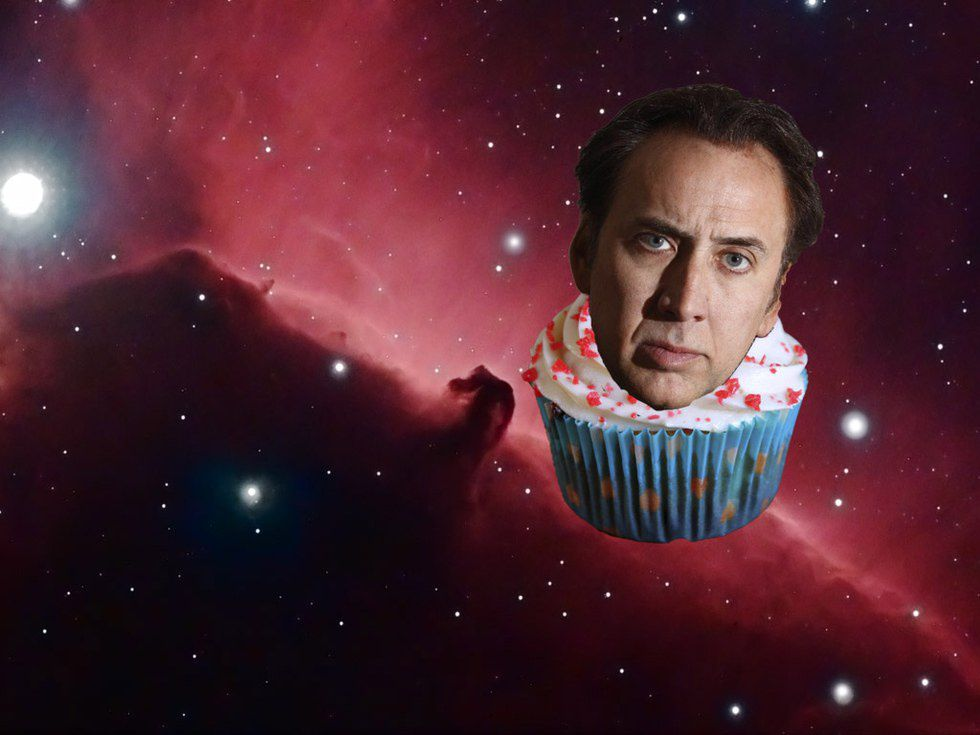
\includegraphics[width=0.4\textwidth]{figures/cupcake1.jpg}
  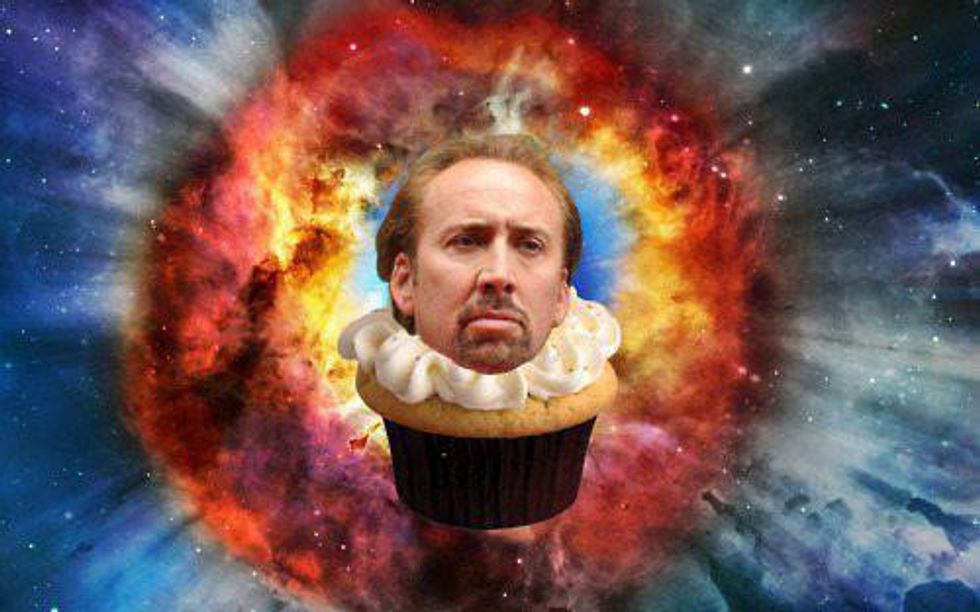
\includegraphics[width=0.4\textwidth]{figures/cupcake2.jpg}
  \caption{Nicolas Cage as a cupcake in space. Figures taken from \citet{reference}.}
  \label{fig:nic_cake}
\end{figure}

\lipsum[41-3]

%% Chapter one

\chapter{Chapter two}
\label{ch:one}

\lipsum[41-50]

 \begin{table}[ht]
\centering
\begin{tabular}{cc}
  \toprule
  \multicolumn{2}{c}{A simple table} \\ \midrule
  1 & 2 \\
  3 & 4 \\
  \bottomrule
\end{tabular}
\caption{A table.} 
\end{table}

\lipsum[51]

%% Conclusions

\epigraphhead[350]{\centering \textit{Fur pillows are hard to actually sleep on.} \\ \textemdash Kanye West}
\part{\label{part:three}Conclusions}

\lipsum[30]

%% List of acronyms
\glsaddall
\renewcommand{\glossarypreamble}{\glsfindwidesttoplevelname[\currentglossary]}
\setglossarystyle{alttree}
\cleardoublepage
\addcontentsline{toc}{chapter}{Acronyms}
\printglossary[type=acronym]

%% List of tables 
\cleardoublepage
\phantomsection
\addcontentsline{toc}{chapter}{Tables}
\listoftables

%% List of figures 
\cleardoublepage
\phantomsection
\addcontentsline{toc}{chapter}{Figures}
\listoffigures

%% Bibliography 
\cleardoublepage
\phantomsection
\addcontentsline{toc}{chapter}{Bibliography}
\printbibliography
\cleardoublepage

\epigraphhead[350]{\centering \textit{I see sounds.} \\ \textemdash Kanye West}
\part{Papers}
\label{papers}
% \includepdf[pages={1-}]{papers/file1.pdf}
% \includepdf[pages={1-}]{papers/file2.pdf}

\end{document}
